\documentclass[]{article}
\usepackage{lmodern}
\usepackage{amssymb,amsmath}
\usepackage{ifxetex,ifluatex}
\usepackage{fixltx2e} % provides \textsubscript
\ifnum 0\ifxetex 1\fi\ifluatex 1\fi=0 % if pdftex
  \usepackage[T1]{fontenc}
  \usepackage[utf8]{inputenc}
\else % if luatex or xelatex
  \ifxetex
    \usepackage{mathspec}
  \else
    \usepackage{fontspec}
  \fi
  \defaultfontfeatures{Ligatures=TeX,Scale=MatchLowercase}
\fi
% use upquote if available, for straight quotes in verbatim environments
\IfFileExists{upquote.sty}{\usepackage{upquote}}{}
% use microtype if available
\IfFileExists{microtype.sty}{%
\usepackage{microtype}
\UseMicrotypeSet[protrusion]{basicmath} % disable protrusion for tt fonts
}{}
\usepackage[margin=1in]{geometry}
\usepackage{hyperref}
\hypersetup{unicode=true,
            pdftitle={Homework 1 - IS 605 FUNDAMENTALS OF COMPUTATIONAL MATHEMATICS},
            pdfauthor={Christophe Hunt},
            pdfborder={0 0 0},
            breaklinks=true}
\urlstyle{same}  % don't use monospace font for urls
\usepackage{color}
\usepackage{fancyvrb}
\newcommand{\VerbBar}{|}
\newcommand{\VERB}{\Verb[commandchars=\\\{\}]}
\DefineVerbatimEnvironment{Highlighting}{Verbatim}{commandchars=\\\{\}}
% Add ',fontsize=\small' for more characters per line
\usepackage{framed}
\definecolor{shadecolor}{RGB}{248,248,248}
\newenvironment{Shaded}{\begin{snugshade}}{\end{snugshade}}
\newcommand{\KeywordTok}[1]{\textcolor[rgb]{0.13,0.29,0.53}{\textbf{{#1}}}}
\newcommand{\DataTypeTok}[1]{\textcolor[rgb]{0.13,0.29,0.53}{{#1}}}
\newcommand{\DecValTok}[1]{\textcolor[rgb]{0.00,0.00,0.81}{{#1}}}
\newcommand{\BaseNTok}[1]{\textcolor[rgb]{0.00,0.00,0.81}{{#1}}}
\newcommand{\FloatTok}[1]{\textcolor[rgb]{0.00,0.00,0.81}{{#1}}}
\newcommand{\ConstantTok}[1]{\textcolor[rgb]{0.00,0.00,0.00}{{#1}}}
\newcommand{\CharTok}[1]{\textcolor[rgb]{0.31,0.60,0.02}{{#1}}}
\newcommand{\SpecialCharTok}[1]{\textcolor[rgb]{0.00,0.00,0.00}{{#1}}}
\newcommand{\StringTok}[1]{\textcolor[rgb]{0.31,0.60,0.02}{{#1}}}
\newcommand{\VerbatimStringTok}[1]{\textcolor[rgb]{0.31,0.60,0.02}{{#1}}}
\newcommand{\SpecialStringTok}[1]{\textcolor[rgb]{0.31,0.60,0.02}{{#1}}}
\newcommand{\ImportTok}[1]{{#1}}
\newcommand{\CommentTok}[1]{\textcolor[rgb]{0.56,0.35,0.01}{\textit{{#1}}}}
\newcommand{\DocumentationTok}[1]{\textcolor[rgb]{0.56,0.35,0.01}{\textbf{\textit{{#1}}}}}
\newcommand{\AnnotationTok}[1]{\textcolor[rgb]{0.56,0.35,0.01}{\textbf{\textit{{#1}}}}}
\newcommand{\CommentVarTok}[1]{\textcolor[rgb]{0.56,0.35,0.01}{\textbf{\textit{{#1}}}}}
\newcommand{\OtherTok}[1]{\textcolor[rgb]{0.56,0.35,0.01}{{#1}}}
\newcommand{\FunctionTok}[1]{\textcolor[rgb]{0.00,0.00,0.00}{{#1}}}
\newcommand{\VariableTok}[1]{\textcolor[rgb]{0.00,0.00,0.00}{{#1}}}
\newcommand{\ControlFlowTok}[1]{\textcolor[rgb]{0.13,0.29,0.53}{\textbf{{#1}}}}
\newcommand{\OperatorTok}[1]{\textcolor[rgb]{0.81,0.36,0.00}{\textbf{{#1}}}}
\newcommand{\BuiltInTok}[1]{{#1}}
\newcommand{\ExtensionTok}[1]{{#1}}
\newcommand{\PreprocessorTok}[1]{\textcolor[rgb]{0.56,0.35,0.01}{\textit{{#1}}}}
\newcommand{\AttributeTok}[1]{\textcolor[rgb]{0.77,0.63,0.00}{{#1}}}
\newcommand{\RegionMarkerTok}[1]{{#1}}
\newcommand{\InformationTok}[1]{\textcolor[rgb]{0.56,0.35,0.01}{\textbf{\textit{{#1}}}}}
\newcommand{\WarningTok}[1]{\textcolor[rgb]{0.56,0.35,0.01}{\textbf{\textit{{#1}}}}}
\newcommand{\AlertTok}[1]{\textcolor[rgb]{0.94,0.16,0.16}{{#1}}}
\newcommand{\ErrorTok}[1]{\textcolor[rgb]{0.64,0.00,0.00}{\textbf{{#1}}}}
\newcommand{\NormalTok}[1]{{#1}}
\usepackage{graphicx,grffile}
\makeatletter
\def\maxwidth{\ifdim\Gin@nat@width>\linewidth\linewidth\else\Gin@nat@width\fi}
\def\maxheight{\ifdim\Gin@nat@height>\textheight\textheight\else\Gin@nat@height\fi}
\makeatother
% Scale images if necessary, so that they will not overflow the page
% margins by default, and it is still possible to overwrite the defaults
% using explicit options in \includegraphics[width, height, ...]{}
\setkeys{Gin}{width=\maxwidth,height=\maxheight,keepaspectratio}
\IfFileExists{parskip.sty}{%
\usepackage{parskip}
}{% else
\setlength{\parindent}{0pt}
\setlength{\parskip}{6pt plus 2pt minus 1pt}
}
\setlength{\emergencystretch}{3em}  % prevent overfull lines
\providecommand{\tightlist}{%
  \setlength{\itemsep}{0pt}\setlength{\parskip}{0pt}}
\setcounter{secnumdepth}{5}
% Redefines (sub)paragraphs to behave more like sections
\ifx\paragraph\undefined\else
\let\oldparagraph\paragraph
\renewcommand{\paragraph}[1]{\oldparagraph{#1}\mbox{}}
\fi
\ifx\subparagraph\undefined\else
\let\oldsubparagraph\subparagraph
\renewcommand{\subparagraph}[1]{\oldsubparagraph{#1}\mbox{}}
\fi

%%% Use protect on footnotes to avoid problems with footnotes in titles
\let\rmarkdownfootnote\footnote%
\def\footnote{\protect\rmarkdownfootnote}

%%% Change title format to be more compact
\usepackage{titling}

% Create subtitle command for use in maketitle
\newcommand{\subtitle}[1]{
  \posttitle{
    \begin{center}\large#1\end{center}
    }
}

\setlength{\droptitle}{-2em}
  \title{Homework 1 - IS 605 FUNDAMENTALS OF COMPUTATIONAL MATHEMATICS}
  \pretitle{\vspace{\droptitle}\centering\huge}
  \posttitle{\par}
  \author{Christophe Hunt}
  \preauthor{\centering\large\emph}
  \postauthor{\par}
  \predate{\centering\large\emph}
  \postdate{\par}
  \date{February 4, 2017}

\usepackage{relsize}
\usepackage{setspace}
\usepackage{amsmath,amsfonts,amsthm}
\usepackage[sfdefault]{roboto}
\usepackage[T1]{fontenc}
\usepackage{float}

\begin{document}
\maketitle

{
\setcounter{tocdepth}{2}
\tableofcontents
}
\section{Problem Set 1}\label{problem-set-1}

\subsection{\texorpdfstring{(1) Calculate the dot product \(u.v\) where
\(u = [0.5; 0.5]~and~v = [3; -4]\)}{(1) Calculate the dot product u.v where u = {[}0.5; 0.5{]}\textasciitilde{}and\textasciitilde{}v = {[}3; -4{]}}}\label{calculate-the-dot-product-u.v-where-u-0.5-0.5andv-3--4}

\begin{Shaded}
\begin{Highlighting}[]
\NormalTok{u <-}\StringTok{  }\KeywordTok{c}\NormalTok{(.}\DecValTok{5}\NormalTok{, .}\DecValTok{5}\NormalTok{)}
\NormalTok{v <-}\StringTok{  }\KeywordTok{c}\NormalTok{(}\DecValTok{3} \NormalTok{,-}\DecValTok{4}\NormalTok{)}

\NormalTok{dotProduct <-}\StringTok{ }\NormalTok{function(x, y)}
\NormalTok{if (}\KeywordTok{length}\NormalTok{(x) !=}\StringTok{ }\KeywordTok{length}\NormalTok{(y))\{}
  \KeywordTok{return}\NormalTok{(}\StringTok{"vectors are not equal lengths"}\NormalTok{)}
  \NormalTok{\} else \{}
    \NormalTok{product <-}\StringTok{ }\KeywordTok{c}\NormalTok{()}
      \NormalTok{for (i in }\DecValTok{1}\NormalTok{:}\KeywordTok{length}\NormalTok{(x))\{}
           \NormalTok{product <-}\StringTok{ }\KeywordTok{append}\NormalTok{(product, (x[[i]] *}\StringTok{ }\NormalTok{y[[i]]))}
       \NormalTok{\}}
  \KeywordTok{return}\NormalTok{(}\KeywordTok{sum}\NormalTok{(product))}
\NormalTok{\}}

\KeywordTok{dotProduct}\NormalTok{(u,v)}
\end{Highlighting}
\end{Shaded}

\begin{verbatim}
## [1] -0.5
\end{verbatim}

\newpage

\subsection{\texorpdfstring{(2) What are the lengths of \(u\) and
\(v\)?}{(2) What are the lengths of u and v?}}\label{what-are-the-lengths-of-u-and-v}

Please note that the mathematical notion of the length of a vector is
not the same as a computer science definition.

\begin{Shaded}
\begin{Highlighting}[]
\NormalTok{u <-}\StringTok{  }\KeywordTok{c}\NormalTok{(.}\DecValTok{5}\NormalTok{, .}\DecValTok{5}\NormalTok{)}
\NormalTok{v <-}\StringTok{  }\KeywordTok{c}\NormalTok{(}\DecValTok{3} \NormalTok{,-}\DecValTok{4}\NormalTok{)}

\KeywordTok{print}\NormalTok{(}\KeywordTok{paste0}\NormalTok{(}\StringTok{"the length of $u$ = "}\NormalTok{, }\KeywordTok{round}\NormalTok{(}\KeywordTok{sqrt}\NormalTok{(}\KeywordTok{dotProduct}\NormalTok{(u,u)), }\DecValTok{2}\NormalTok{)))}
\end{Highlighting}
\end{Shaded}

{[}1{]} ``the length of \(u\) = 0.71''

\begin{Shaded}
\begin{Highlighting}[]
\KeywordTok{print}\NormalTok{(}\KeywordTok{paste0}\NormalTok{(}\StringTok{"the length of $v$ = "}\NormalTok{, }\KeywordTok{round}\NormalTok{(}\KeywordTok{sqrt}\NormalTok{(}\KeywordTok{dotProduct}\NormalTok{(v,v)), }\DecValTok{2}\NormalTok{)))}
\end{Highlighting}
\end{Shaded}

{[}1{]} ``the length of \(v\) = 5''

\subsection{\texorpdfstring{(3) What is the linear combination:
\(3u - 2v\)?}{(3) What is the linear combination: 3u - 2v?}}\label{what-is-the-linear-combination-3u---2v}

\begin{Shaded}
\begin{Highlighting}[]
\NormalTok{u <-}\StringTok{  }\KeywordTok{c}\NormalTok{(.}\DecValTok{5}\NormalTok{, .}\DecValTok{5}\NormalTok{)}
\NormalTok{v <-}\StringTok{  }\KeywordTok{c}\NormalTok{(}\DecValTok{3} \NormalTok{,-}\DecValTok{4}\NormalTok{)}

\NormalTok{linearCombo <-}\StringTok{ }\NormalTok{function(xMulti, x, yMulti, y, }\DataTypeTok{subtract =} \OtherTok{TRUE}\NormalTok{)\{}
      \NormalTok{xResults  <-}\StringTok{ }\KeywordTok{c}\NormalTok{()}
      \NormalTok{yResults  <-}\StringTok{ }\KeywordTok{c}\NormalTok{()}
      \NormalTok{linCombo <-}\StringTok{ }\KeywordTok{c}\NormalTok{()}
    \NormalTok{for (i in }\DecValTok{1}\NormalTok{:}\KeywordTok{length}\NormalTok{(x))\{  }
      \NormalTok{xResults <-}\StringTok{ }\KeywordTok{append}\NormalTok{(xResults, (xMulti *}\StringTok{ }\NormalTok{x[[i]]))}
    \NormalTok{\}}
    \NormalTok{for (i in }\DecValTok{1}\NormalTok{:}\KeywordTok{length}\NormalTok{(y))\{ }
      \NormalTok{yResults <-}\StringTok{ }\KeywordTok{append}\NormalTok{(yResults, (yMulti*}\StringTok{ }\NormalTok{y[[i]]))}
    \NormalTok{\}}
    \NormalTok{if (subtract ==}\StringTok{ }\OtherTok{TRUE}\NormalTok{)\{ }
    \NormalTok{for (i in }\DecValTok{1}\NormalTok{:}\KeywordTok{length}\NormalTok{(xResults))}
      \NormalTok{linCombo <-}\StringTok{ }\KeywordTok{append}\NormalTok{(linCombo, (xResults[[i]] -}\StringTok{ }\NormalTok{yResults[[i]]))}
    \NormalTok{\} else \{}
    \NormalTok{for (i in }\DecValTok{1}\NormalTok{:}\KeywordTok{length}\NormalTok{(xResults))}
      \NormalTok{linCombo <-}\StringTok{ }\KeywordTok{append}\NormalTok{(linCombo, (xResults[[i]] -}\StringTok{ }\NormalTok{yResults[[i]]))}
    \NormalTok{\}}
    \KeywordTok{return}\NormalTok{(linCombo)}
\NormalTok{\}}

\NormalTok{x <-}\StringTok{ }\KeywordTok{linearCombo}\NormalTok{(}\DataTypeTok{xMulti =} \DecValTok{3}\NormalTok{, u, }\DataTypeTok{yMulti =} \DecValTok{2}\NormalTok{, v)}

\KeywordTok{paste0}\NormalTok{(}\StringTok{"["}\NormalTok{,x[}\DecValTok{1}\NormalTok{], }\StringTok{" , "} \NormalTok{, x[}\DecValTok{2}\NormalTok{], }\StringTok{"]"}\NormalTok{)}
\end{Highlighting}
\end{Shaded}

\begin{verbatim}
## [1] "[-4.5 , 9.5]"
\end{verbatim}

\subsection{\texorpdfstring{(4) What is the angle between \(u\) and
\(v\)}{(4) What is the angle between u and v}}\label{what-is-the-angle-between-u-and-v}

\begin{Shaded}
\begin{Highlighting}[]
\NormalTok{angle <-}\StringTok{ }\KeywordTok{acos}\NormalTok{((}\KeywordTok{dotProduct}\NormalTok{(u,v) /}\StringTok{ }\NormalTok{(}\KeywordTok{sqrt}\NormalTok{(}\KeywordTok{dotProduct}\NormalTok{(u,u)) *}\StringTok{ }\KeywordTok{sqrt}\NormalTok{(}\KeywordTok{dotProduct}\NormalTok{(v,v)))))}
\NormalTok{angle}
\end{Highlighting}
\end{Shaded}

\begin{verbatim}
## [1] 1.712693
\end{verbatim}

\section{Problem Set 2}\label{problem-set-2}

Set up a system of equations with 3 variables and 3 constraints and
solve for x. Please write a function in R that will take two variables
(matrix A \& constraint vector b) and solve using elimination. Your
function should produce the right answer for the system of equations for
any 3-variable, 3-equation system. You don't have to worry about
degenerate cases and can safely assume that the function will only be
tested with a system of equations that has a solution. Please note that
you do have to worry about zero pivots, though. Please note that you
should not use the built-in function solve to solve this system or use
matrix inverses. The approach that you should employ is to construct an
Upper Triangular Matrix and then back-substitute to get the solution.
Alternatively, you can augment the matrix A with vector b and jointly
apply the Gauss Jordan elimination procedure.

\begin{figure}
\centering
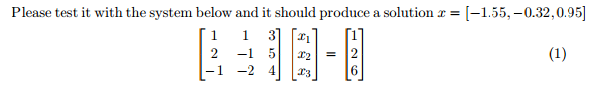
\includegraphics{https://raw.githubusercontent.com/ChristopheHunt/MSDA---Coursework/master/Data\%20605/Assignment\%201/problemset2.PNG}
\caption{img}
\end{figure}


\end{document}
